\chapter{Introduction}\label{introduction}

\epigraph{The labour of the astronomer in the present state of his art is much like that of one who should examine, grain by grain, the sands of the sea in the certainty that among them numerous grains must exist of extraordinary value\dots}{-- Sir John Herschel\footnotemark}

\footnotetext{\emph{Memoirs of the Royal Astronomical Society.} 1826, Vol.\ 2, p472}


\section{The first of many sections}

Lorem ipsum dolor sit amet, consectetur adipiscing elit. Duis posuere tellus eu quam pellentesque ut varius purus egestas. Nam hendrerit malesuada sapien, non molestie risus cursus at. Pellentesque habitant morbi tristique senectus et netus et malesuada fames ac turpis egestas. Sed dignissim sodales sem sed volutpat. Ut laoreet, ante sed dictum vestibulum, lacus sapien semper dui, nec rutrum velit justo eu enim. Fusce vehicula blandit ipsum, ac volutpat libero vestibulum in. Sed quis lacus mauris. Quisque congue elit in nisi lacinia ac condimentum eros pellentesque. Quisque et nisl odio, vitae eleifend neque. Oh look, a sneaky citation to my paper \citep[][of which I am a co-author]{Kastner12}.


Phasellus erat libero, lobortis vitae iaculis nec, congue et tortor. Donec tempus leo et nisl tincidunt porta. Nulla velit sapien, sollicitudin sit amet accumsan a, facilisis a est. Phasellus scelerisque convallis sapien, nec viverra dui tincidunt a. Nulla ligula velit, laoreet fringilla condimentum sed, euismod a est. Fusce leo sapien, rhoncus a ultricies nec, porttitor ut lectus. Sed vestibulum turpis risus, nec vestibulum diam. Morbi quis quam quis enim cursus aliquam scelerisque quis tellus. Pellentesque accumsan lectus cursus massa ultrices placerat. Nulla facilisi. Praesent fermentum erat in augue sagittis condimentum. Nullam posuere blandit urna a mollis. Cras malesuada lectus a turpis sollicitudin volutpat. Morbi semper, nisl vel mattis vehicula, sapien sapien adipiscing tortor, in accumsan tortor dolor non neque. Maecenas varius, nunc ut euismod volutpat, mauris ante faucibus magna.

\subsection{A subsection}

Vestibulum sed orci nec diam euismod vehicula vitae et mauris. Phasellus sagittis justo quis mauris adipiscing auctor. Suspendisse nibh erat, cursus vitae aliquam in, rutrum sed est. Nunc mollis quam quis velit vehicula fringilla. Quisque convallis, neque ut faucibus luctus, nisl ante porttitor ante, at venenatis lectus nulla sed augue. Quisque lacinia semper lacus, nec ultricies justo auctor vel. Aenean viverra aliquam est ac porttitor.

% THIS FIGURE USES THE \echa MACRO DEFINED IN macros.tex
\begin{figure}[t!]
\vspace{-4mm}
   \centering
   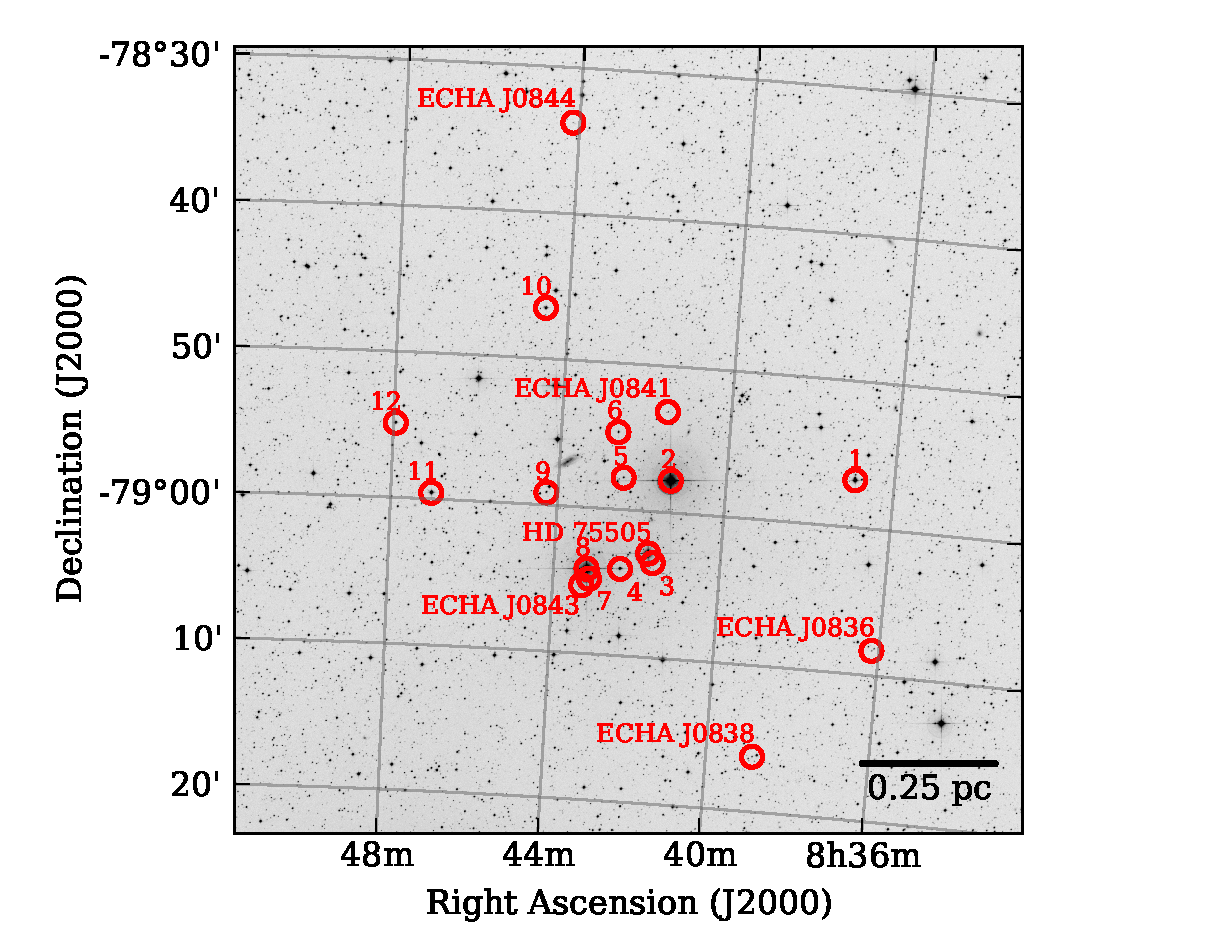
\includegraphics[width=\textwidth]{etacha} 
   \caption[{The \object[ETA CHA CLUSTER]{$\eta$ Chamaeleontis} open cluster}]{$0.9\times0.9$~deg DSS2-IR image showing the 18 member systems of the \echa\ cluster. The bright star at the centre of the image is the eponymous \echa. The bar shows the linear scale at the 94.3~pc cluster distance.}
   \label{fig:etacha}
\end{figure}

\section{Wow, another section heading!}

Sed tempor imperdiet rhoncus. Cras mi neque, pellentesque ac ultricies vitae, feugiat ut ante. Suspendisse vestibulum venenatis odio, quis pharetra mauris dapibus in. Pellentesque sagittis laoreet mi sed vestibulum. Ut iaculis venenatis urna eu tincidunt. Duis consequat est ut velit rutrum vitae placerat dolor eleifend. Nullam eget nulla massa, non accumsan libero. Sed auctor velit bibendum nisl tincidunt aliquam. Aenean pellentesque eros a lectus imperdiet rhoncus. Another citation to one of my papers \citep{Riedel11}.

Nunc non odio leo. Phasellus sodales pretium nunc suscipit bibendum. Nullam lorem turpis, varius sed bibendum id, interdum sed lectus. Ut rutrum, orci in adipiscing accumsan, velit massa dapibus metus, id volutpat nulla eros eget lorem. Ut massa massa, ornare vitae elementum ut, consequat a justo. Vestibulum tempus fermentum commodo. In vel auctor nisi. Mauris id turpis nisi. Nulla eget magna eu magna rhoncus pulvinar. Morbi enim ligula, feugiat et rutrum in, posuere eget lacus. Suspendisse adipiscing, erat in hendrerit dictum, est tellus vestibulum justo, et sodales mi dolor sed purus.

In porttitor purus et metus adipiscing molestie. Curabitur scelerisque, sem ac sodales sodales, neque metus commodo massa, eu pulvinar ante lectus eu orci. Mauris non odio vel enim scelerisque porttitor ac ac lacus. Pellentesque habitant morbi tristique senectus et netus et malesuada fames ac turpis egestas. Phasellus id dolor dui. Cras non neque vel turpis posuere commodo et nec leo. Nulla dictum rutrum nisi ac rhoncus. Aenean lobortis tempor magna viverra iaculis. Ut sit amet nunc mi. Integer iaculis condimentum diam non dignissim. Duis bibendum auctor velit id scelerisque.

Nulla tincidunt tortor ac odio posuere eget semper mauris tristique. Vestibulum congue magna sed arcu tincidunt id pharetra nisi hendrerit. Duis erat nulla, fringilla sed tempus at, sodales a libero. Nunc ullamcorper dapibus dui, ut varius tellus ullamcorper quis. Pellentesque odio lacus, molestie quis porta vitae, ornare eget massa. Integer hendrerit sapien ac massa lobortis in malesuada quam dignissim. Aliquam feugiat, nisl ut semper auctor, purus nunc iaculis ipsum, non tristique nibh felis a ipsum. Pellentesque odio lacus, molestie quis porta vitae, ornare eget massa. Ut sit amet nunc mi. Integer iaculis condimentum diam non dignissim. Duis bibendum auctor velit id scelerisque.

You can click on objects and be taken to their SIMBAD entry, like this: \object{Large Magellanic Cloud}. All of the objects in Table~\ref{table:etacha} are resolvable in SIMBAD.

% I think ctable gives the best LaTeX tables, once you get to know its syntax. All of the objects in this table are resolvable in SIMBAD using the \object{} command defined in macros.tex

\ctable[caption={Census of the \object[ETA CHA CLUSTER]{$\eta$ Chamaeleontis cluster} prior to this work},label=table:etacha,doinside=\small \setlength{\extrarowheight}{0pt}
,captionskip=0pt,pos=b]{lcccccccc}
{\tnote[$\dagger$]{\citet{Murphy10} (K and M members), \citet{Murphy11} (early-type members)}
\tnote[$\ddag$]{Photometry from \citet{Bessell12}}
\tnote[$\star$]{\object[ECHA J0844.2-7833]{ECHA J0844.2} has an elevated position in the cluster CMD}
}{
\toprule[2pt]
Name & Right Ascension & Declination & Spectral & $V$\tmark[$\ddag$] & Binary?\tmark[$\star$]\\
 & [J2000 deg] & [J2000 deg] & Type\tmark[$\dagger$] & [mag]\\
\midrule
 \object[ECHA J0836.2-7908]{ECHA J0836.2$-$7908} & 08 36 10.6 & $-$79 08 18 & M5.3 & 17.66 & suspected\\
  \object{RECX 1} & 08 36 56.2 & $-$78 56 46 & K7.0 & 10.61 & yes\\
  \object[ECHA J0838.9-7916]{ECHA J0838.9$-$7916} & 08 38 51.5 & $-$79 16 14 & M5.0 & 16.82 & suspected\\
  \object[ETA CHA]{$\eta$ Cha} (\object{RECX 2}) & 08 41 19.5 & $-$78 57 48 & B8V & 5.46& suspected\\
  \object[ECHA J0841.5-7853]{ECHA J0841.5$-$7853} & 08 41 30.6 & $-$78 53 07 & M4.7 & 17.07 & \\
  \object{RECX 3} & 08 41 37.2 & $-$79 03 31 & M3.0 & 14.35 \\
  \object{HD 75505} & 08 41 44.7 & $-$79 02 53 & A6 & 7.27\\
  \object{RECX 4} & 08 42 23.7 & $-$79 04 04 & M1.3 & 12.79\\
  \object{RECX 5} & 08 42 27.3 & $-$78 57 49 & M3.8 & 15.20\\
  \object{RECX 6} & 08 42 39.0 & $-$78 54 44 & M3.0 & 14.08\\
  \object{RECX 7} & 08 43 07.7 & $-$79 04 52 & K6.9 & 10.84 & yes\\
  \object{RS Cha} (\object{RECX 8}) & 08 43 12.2 & $-$79 04 12 & A8V+A8V & 6.28 & triple?\\
  \object[ECHA J0843.3-7905]{ECHA J0843.3$-$7905} & 08 43 18.4 & $-$79 05 21 & M3.4 & 13.97\\
  \object[ECHA J0844.2-7833]{ECHA J0844.2$-$7833} & 08 44 09.1 & $-$78 33 46 & M5.5 &  & suspected\\
  \object{RECX 9} & 08 44 16.6 & $-$78 59 09 & M4.4 & 15.00 & yes\\
  \object{RECX 10} & 08 44 32.2 & $-$78 46 32 & M0.3 & 12.53\\
  \object{RECX11} & 08 47 01.8 & $-$78 59 35 & K6.5 & 11.13\\
  \object{RECX 12} & 08 47 56.9 & $-$78 54 54 & M3.2 & 13.17 & suspected\\
\bottomrule[2pt]
}

